% !TeX root = ../libro.tex
% !TeX encoding = utf8

\chapter{Desarrollo e implementación}
En esta sección veremos cómo se han usado las técnicas y conceptos presentados para la realización de una aplicación web que permita al usuario crear e interactuar superficies a través de SDFs, ecuaciones implícitas y paramétricas. El motivo de desarrollar una aplicación web es que sea accesible al mayor número de usuarios y de la forma más cómoda posible. Se ha decidido usar \href{https://es.reactjs.org/}{React} para esta tarea, una biblioteca de JavaScript (y TypeScript) para interfaces de usuario. Es una librería muy popular, y por tanto muy bien documentada y con muchos paquetes de la comunidad disponibles. Las principales características de React son:
\begin{itemize}
    \item Utiliza la \textbf{extensión de sintaxis} JSX, la cual permite escribir código JavaScript como si se tratase de HTML o XML. Se pueden usar expresiones JSX dentro de bucles \texttt{for} o entornos condicionales \texttt{if}, y dentro de ellas se pueden agregar expresiones JS entre corchetes. 
    \item Se basa en \textbf{componentes autocontenidos y reutilizables}. La forma más común actualmente de declarar componentes es a través de funciones que reciben argumentos, o \texttt{props}, y devuelven una expresión JSX. Todos los componentes reciben el parámetro \texttt{children} por defecto, conteniendo la expresión JSX de los componentes que se encuentren entre las etiquetas de apertura y cierre del componente. El flujo de datos es unidireccional del componente padre a sus hijos.
    \item Utiliza un \textbf{DOM virtual} para solo actualizar los componentes cuyo estado o \texttt{props} han cambiado. En componentes funcionales, la manera de indicar variables que desencadenen un re-renderizado al ser modificadas es a través de \textit{hooks}. En general, estos son funciones de JS que permiten crear y acceder al estado y ciclos de vida de React. Los principales son \texttt{useState}, usado para declarar una variable junto con su \textit{setter}, y \texttt{useEffect}, que permite ejecutar código cuando se actualice el componente. Si solo se quiere reaccionar a cambios de ciertos \textit{hooks} se puede indicar en las dependencias.
\end{itemize}
Un ejemplo de uso básico de JSX, componentes funcionales y manejo de estado sería el siguiente:
\begin{lstlisting}
function Tarjeta(props) {
  return (
    <div>
        {props.children}
        {props.nombre}
    </div>
  );
}

function Main() {
    const [miNombre, setMiNombre] = React.useState("Daniel");

    useEffect(()=>{
        console.log("Solo me ejecuto una vez al inicio");
    }, []);
    
    useEffect(()=>{
        console.log("Has cambiado el nombre");
    }, [miNombre]);
    
  return (
    <TarjetaNombre nombre={miNombre}>
      <h1>Hola, mi nombre es</h1>
    </TarjetaNombre>
  );
}
\end{lstlisting}
Las principales ventajas que nos aportará el uso de React son las siguientes.
\begin{itemize}
    \item La aplicación puede ser ejecutada en cualquier navegador, haciendo que sea mucho más accesible.
    \item Está basada en componentes modulares, lo que la hace escalable. Además. debido a su popularidad, hay una infinidad de librerías de terceros a nuestra disposición, ya sea específicas de React o de JavaScript.
\end{itemize}

% Un aspecto fundamental a lo largo de todo el desarrollo será el del rendimiento ya que las aplicaciones web solo tienen a su disposición una hebra de ejecución (la de interfaz de usuario), haciendo de cuello de botella para el resto de cálculos.\newline

La aplicación consta de tres componentes principales. Dos de ellos son con los que interactúa el usuario, uno en la que se le permite crear primitivas introduciendo directamente una SDF, ecuaciones implícitas o paramétricas, y otro que contiene un editor de nodos en forma de árbol para aplicar operaciones sobre las primitivas creadas y guardar los resultados obtenidos. El último componente actúa como gestor de almecenamiento y estado de la aplicación. A continuación estudiamos cada componente por separado describiendo los subcomponentes que la conforman y cómo estos interaccionan entre sí.

\section{Gestor de estado}
Empezamos hablando sobre el gestor de estado, ya que el resto de componentes dependen y se comunican entre sí a través de este. Para esta tarea se ha hecho uso de \href{https://github.com/pmndrs/zustand}{Zustand}, un paquete de gestión de estado para JavaScript. Con él se pueden crear contenedores formados por atributos y métodos para gestionarlos. Cuando un componente quiere acceder a un contenedor, basta con que se suscriba a sus cambios a través del \textit{hook} que proporciona Zustand: \texttt{useStore}. Nosotros haremos uso de dos contenedores, uno para las primitivas definidas y otro para gestionar el estado del editor de nodos. De este último hablaremos en la siguiente sección, pues solo es usado por el componente del editor de nodos. Sin embargo el contenedor de primitivas es usado tanto por el editor de nodos como por el creador de primitivas, ya que ambos deben leer de él para saber cuales son las primitivas existentes y pueden escribir para crear una nueva primitiva. Este contenedor tiene la estructura mostrada en la \autoref{fig:contenedorPrim}. En particular, la información se almacena a través del tipo \texttt{Primitive}, el cual tiene los siguientes atributos.
\begin{itemize}
    \item \texttt{id}: identificador único obtenido aplicando normalización NFD al nombre de la primitiva que introduce el usuario.
    \item \texttt{name}: nombre que otorga el usuario a la primitiva y será mostrado por pantalla.
    \item \texttt{inputMode}: indica el método que usó el usuario para definir la primitiva, ya sea introduciendo directamente la SDF con sintaxis GLSL, la ecuación implícita o la parametrización racional.
    \item \texttt{input}: cadena de texto con la ecuación introducida por el usuario. En el caso de las parametrizaciones se guarda por separado cada ecuación.
    \item \texttt{sdf}: función distancia con signo obtenida tras procesar la entrada del usuario.
    \item \texttt{parameters}: parámetros asociados a la primitiva definidos por el usuario, que podrán ser usados en el editor de nodos. A su vez, el tipo \texttt{Parameter} contiene el símbolo del parámetro presente en la expresión, una etiqueta para ser mostrado en el editor de nodos, y si su valor debe estar acotado en cierto rango. 
    \item \texttt{fHeader}: cabecera de la función GLSL asociada a la primitiva. La función recibe como nombre el \texttt{id}, y recibe como argumentos el punto donde se quiera evaluar la SDF y los definidos por el usuario.
    \item \texttt{material}: contiene las componentes especular, difusa y ambiental y el coeficiente de brillo del material asociado a la primitiva.
\end{itemize}
\begin{ejemplo}
Para definir una esfera centrada en el origen mediante su ecuación implícita y poder controlar su radio en el editor de nodos, se crearía la siguiente primitiva.
\begin{lstlisting}
{
  id: "sphere",
  name: "Sphere",
  inputMode: InputMode.Implicit,
  input: ["x^2 + y^2 + z^2 - r", "", ""],
  parsedInput: "length(p)-r",
  parameters: [
     { symbol: "r", label: "Radius", defaultVal: 1.0, type: "range", range:[0,100] }
  ],
  fHeader: "sphere(vec3 p, float r)",
  material: {
    specular: [1.0, 1.0, 1.0],
    diffuse: [0.0, 1.0, 0.0],
    ambient: [0.2, 0.2, 0.2],
    smoothness: 10.0
  }
}
\end{lstlisting}
\end{ejemplo}

\begin{figure}[ht!]
    \centering
    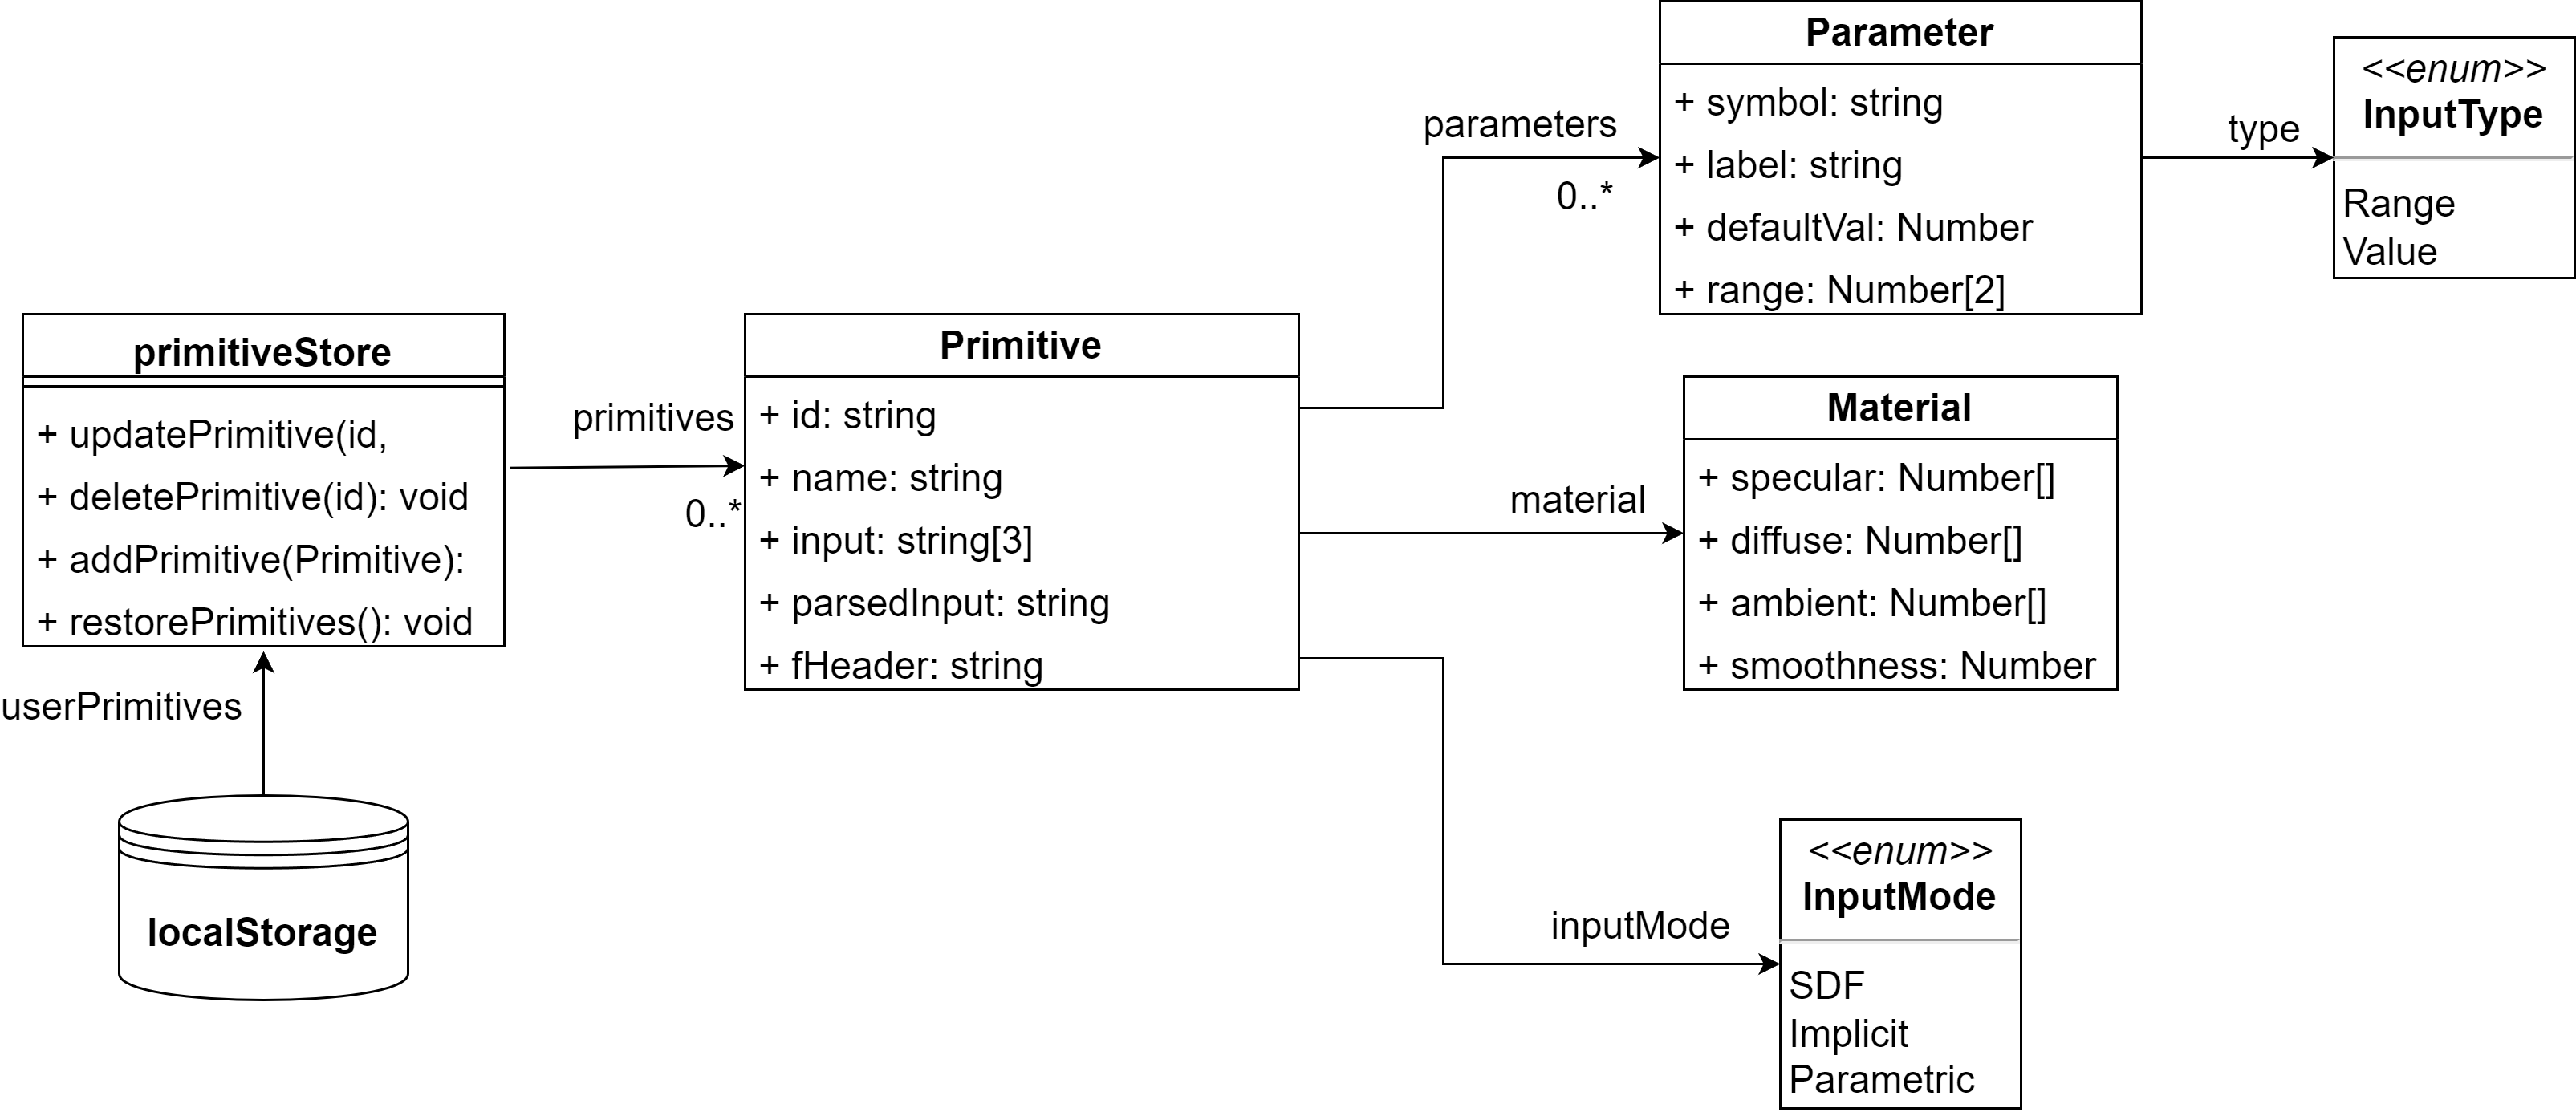
\includegraphics[width=\textwidth]{Plantilla-TFG-master/img/diagramaZustand.png}
    \caption{Diagrama de clases del contenedor de primitivas}
    \label{fig:contenedorPrim}
\end{figure}

Las principales ventajas de la elección de Zustand es que se trata de una biblioteca de tamaño muy pequeño, y al estar basada en \textit{hooks} solo actualizará los componentes que dependan de los cambios relevantes en el estado, haciendo la aplicación más eficiente. Además, al ser la única forma de acceder a los datos a través de los métodos del contenedor, es más fácil debugear y evitar que haya modificaciones inesperadas desde algún componente externo. Por último, es muy sencillo almacenar el estado del contenedor en el almacenamiento local, de forma que el usuario pueda disponer de los datos guardados en sesiones anteriores.


\section{Editor de nodos}
Este componente se basa en \href{https://github.com/wbkd/react-flow}{React Flow}, un paquete muy completo que permite la implementación de diagramas interactivos basados en nodos. Cada nodo tendrá cierto número de puertos de entrada (solo permite la conexión con un nodo) y uno de salida (permite conectarse a varios nodos). Se nos permite declarar tipos de nodos según nuestras necesidades. Nosotros usaremos dos categorías principales de nodos.\newline

El primer tipo es el \textbf{nodo de primitiva}. Es el más sencillo y permite seleccionar una primitiva entre las guardadas para ser conectada a uno o varios nodos de operaciones.\newline

Los \textbf{nodos de operaciones} implementan las operaciones explicadas en la \autoref{sec:operaciones} y las aplican a las primitivas que reciben por sus puertos de entrada. A su vez hay cuatro tipos diferentes de estos nodos, uno por cada tipo de operación. Los nodos de operaciones de transformación, deformación y repetición tienen un único puerto de entrada, pues son operadores unarios. El nodo booleano sin embargo es capaz de recibir un número arbitrario de primitivas, ya que aunque los operadores booleanos son binarios, si se quiere realizar una misma operación de forma reiterada sobre varias primitivas puede ser muy tedioso. Así, si un nodo booleano recibe las primitivas $A_i$ con $i=1,\dots, n$, irá aplicando la operación de forma sucesiva sobre el resultado anterior según el orden de conexión. Por ejemplo, para la unión tendríamos
\begin{equation*}
    \bigcup_{i=0}^n A_i = A_n\bigcup (A_{n-1} \bigcup ( \cdots A_2 \bigcup A_1)).
\end{equation*}

La estructura de todos los nodos es similar. Todos cuentan con un encabezado que muestra de qué tipo son, un desplegable para elegir la primitiva u operación a usar seguido de un área con controles para los parámetros que puedan tener, un lienzo para mostrar el resultado de las operaciones aplicadas hasta el momento, y un botón para contraer el nodo ocultando toda la información excepto el encabezado. Debido a esto tiene sentido tener un componente nodo general que se pueda adaptar a diferentes tipos de uso. El encabezado y elementos del desplegable se pasan fácilmente a través de \texttt{props}. Sin embargo para los parámetros sí que dependen fuertemente del tipo de nodo en particular, y serán implementados por cada tipo de nodo por separado y pasado al general a través del parámetro \texttt{children}.\newline

De manera interna React Flow usa Zustand para almacenar la información relativa a los identificadores de los nodos, sus posiciones, conexiones, etc. Nosotros extenderemos esta funcionalidad para poder usar el modelo de generación de superficies en forma de árbol presentado en la \autoref{sec:operaciones}. Para ello bastará con almacenar para cada nodo la información relativa a su SDF actual, sus entradas y sus nodos hijo (padres), así como funciones para gestionar los nodos (añadir, eliminar, actualizar, conectar, etc.). Mediante estas operaciones, cuando un nodo detecta una nueva conexión en algún puerto de entrada se leen las SDFs de los nodos conectados, y junto con los propios parámetros del nodo se actualiza la SDF del nodo. Cuando se elimina alguna conexión en el caso de los nodos diferentes al booleano simplemente la SDF pasa a ser indefinida, ya que solo tienen una entrada. En el caso del booleano habrá que tener en cuenta si todavía queda alguna entrada, reorganizar las restantes para que no haya puertos vacíos distintos al último, y reducir el número de puertos a uno menos. Para esto, se detecta la posición del puerto que se ha eliminado y se modifican las conexiones siguientes para cambiar su puerto al inmediatamente anterior. 
\begin{figure}[!h]
    \centering
    \begin{subfigure}[b]{0.45\textwidth}
        \centering
        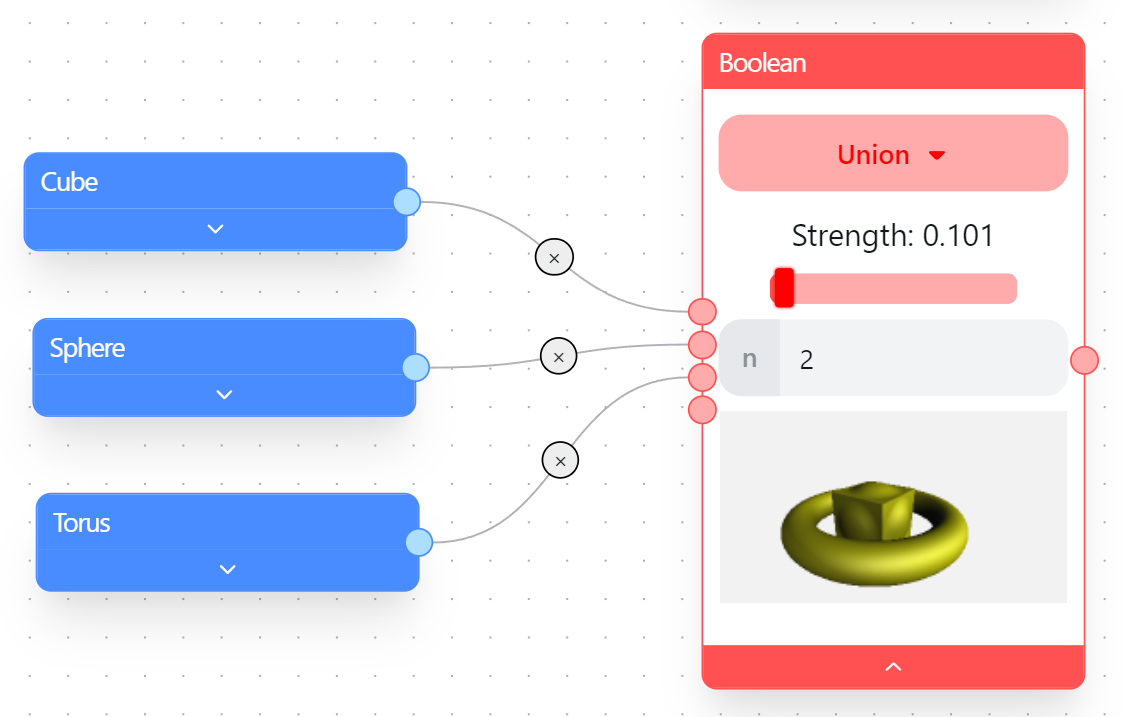
\includegraphics[width=\textwidth]{Plantilla-TFG-master/img/booleanBorrar1.png}
        \caption{Antes de eliminar}
    \end{subfigure}
    \hspace{15pt}
    \begin{subfigure}[b]{0.45\textwidth}
        \centering
        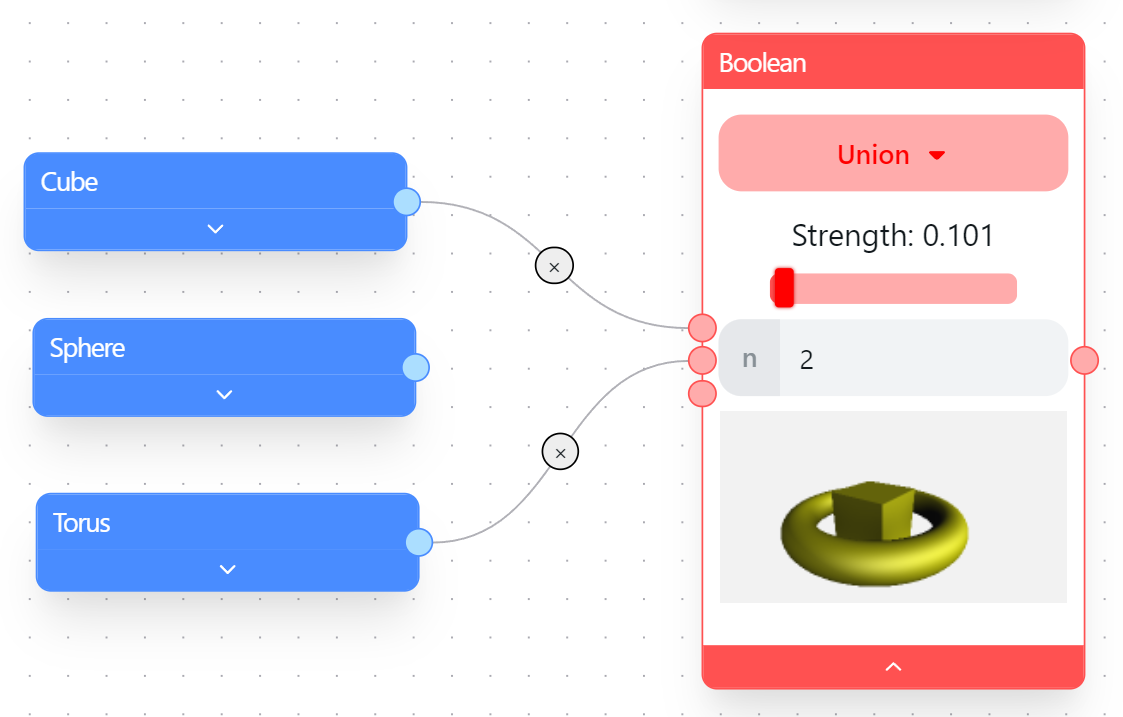
\includegraphics[width=\textwidth]{Plantilla-TFG-master/img/booleanBorrar2.png}
        \caption{Tras eliminar segunda conexión}
    \end{subfigure}
    \hfill
     \caption{Ejemplo de eliminación de conexión en nodo booleano}
\end{figure}

Para poder visualizar los efectos que tienen las acciones del usuario cada nodo tiene una instancia de un componente \texttt{Shader}. Este componente consta de un lienzo creado con \href{https://github.com/gre/gl-react}{gl-react} y que recibe como parámetro una SDF para renderizarla usando \textit{spheretracing} como se explicó en la \autoref{sec:render}, aplicando los algoritmos de iluminación y sombras de la \autoref{sec:ilum}. Se pasan los siguientes \texttt{uniforms} al \textit{fragment shader} del lienzo: 
\begin{itemize}
    \item Material de la primitiva con la estructura mostrada en la \autoref{fig:contenedorPrim} a través de varios \texttt{vec3} y \texttt{float}. 
    \item Resolución del lienzo en píxeles como un \texttt{vec2}.
    \item La dirección, color y tamaño de las luces como \texttt{float[]} agrupados de tres en tres en el caso de la dirección y el color. Dado que GLSL solo admite arrays de longitud fija, se ha fijado el número de luces en cuatro, aunque por defecto solo se utilizan dos al igual que en el ejemplo de la \autoref{sec:ilum},
    \item Dos ángulos como un \texttt{vec2} y una distancia como \texttt{float} actuando como coordenadas esféricas del observador respecto al origen. Ambos parámetros se controlan por el usuario a través del ratón.
\end{itemize}

\section{Panel de primitivas}
En esta sección el usuario será capaz de visualizar y modificar las primitivas existentes, así como crear nuevas. Para ello se presenta una tabla que muestra la información más relevante de las primitivas presentes en el contenedor de Zustand, incluyendo en cada fila botones para editar o eliminar cada primitiva. En el caso de que se desee eliminar alguna, bastará con llamar a la función correspondiente del contenedor. Si en cambio se desea realizar una modificación, se abrirá un cuadro de diálogo con toda la información de la primitiva, incluyendo los parámetros y ecuaciones que introdujo el usuario en el momento de la creación (razón por la cual guardábamos esta información en el contenedor) y el método de definición de la superficie (a través de una ecuación implícita, parametrización o SDF). En todo momento se comprueba que el usuario esté introduciendo información válida, y en caso contrario se le notifica del error en el campo correspondiente. Algunos comprobaciones de vital importancia son las siguientes.
\begin{itemize}
    \item Dado que el identificador se calcula a partir del nombre que introduzca el usuario, no se podrá elegir ningún nombre cuyo identificador asociado ya esté asignado a otra primitiva diferente.
    \item No se pueden utilizar parámetros que no estén correctamente definidos en la tabla correspondiente. De darse el caso, se le indicará al usuario la ecuación que contiene el error y el símbolo en cuestión.
    \item Cuando se introduce directamente la SDF mediante sintaxis GLSL, la expresión debe ser sintácticamente correcta. En caso de error, para ser capaces de identificar su motivo deberemos instalar un centinela o \texttt{Visitor} en el componente \texttt{Shader}, de forma que cuando este detecte un error de compilación sea capaz de capturarlo y procesarlo para transmitirlo de forma natural al usuario.
    \item Al introducir una ecuación implícita, dado que para calcular la SDF se utiliza la \autoref{p:aproxImp}, deberemos comprobar que la norma del gradiente no es cero.
    \item Se usan las variables adecuadas en cada caso: $x,y,z$ en el caso de ecuaciones implícitas y $s,t$ para las parametrizaciones. 
\end{itemize}
En la siguiente sección se verá con más detalle como se realizan las comprobaciones relativas a la validez de las ecuaciones.\newline

Una vez toda la información introducida es válida, se le permite al usuario pulsar el botón de guardar. Esta acción hará que se llame a la función del contenedor de primitivas correspondiente, haciendo que se sobreescriba la primitiva original y se reflejen los cambios tanto en el editor de nodos como en la tabla de primitivas. Por último, en caso de que el usuario quiera crear una primitiva, el funcionamiento interno es el mismo, con la única excepción de que el cuadro de dialogó aparecerá completamente vacío.

\section{Librería de polinomios multivariable}
Si bien tenemos a nuestra disposición un gran número de librerías externas, en el momento de realización de la aplicación no se encontró ninguna opción viable para trabajar con polinomios multivariable en JavaScript de forma nativa. Como alternativas se barajó el uso de la API de \href{https://wiki.geogebra.org/en/Reference:GeoGebra_Apps_API}{Geogebra} o realizar llamadas a código Python que usara \href{https://www.sagemath.org/}{SageMath}. Sin embargo, por motivos de rendimiento y completitud de este trabajo, se decidió desarrollar una librería nativa en TypeScript para el manejo de polinomios en varias variables y cálculo de bases de Gröbner. Se encuentra disponible en \href{https://github.com/Daniel2000815/multivariate-polynomial}{GitHub} junto a su documentación, ejemplos de uso y tests usados. La librería consta de tres clases principales que pasamos a estudiar a continuación.

\subsection{Clase \texttt{Monomial}}

\subsection{Clase \texttt{Polynomial}}

\subsection{Clase \texttt{Ideal}}